\documentclass[usenames,dvipsnames,tikz]{standalone}
\usepackage{amsmath,amssymb}
\usepackage{xcolor}
\colorlet{tBlue}{RoyalBlue!35!Cerulean}
\colorlet{tRed}{Red}
\usepackage{tikz}
\usepackage{standalone}
\begin{document}
	
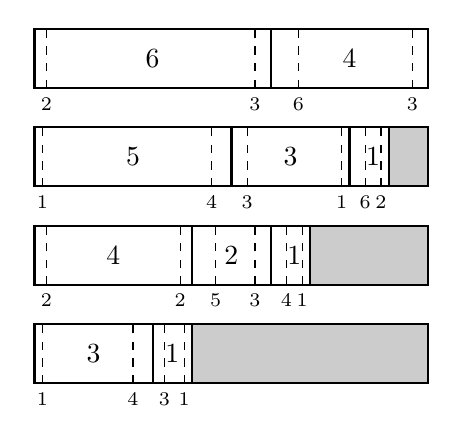
\begin{tikzpicture}
%\draw [help lines] (-1,-2) grid (13,5);
% 1=0.1, 2=0.15, 3=0.2, 4=0.25, 5=0.3
% 6, 5, 4, 4, 3, 3, 2, 1, 1, 1.

%---------------------------------------------------------------------
% SCPP
% 1=0.1, 2=0.15, 3=0.2, 4=0.25, 5=0.3
\draw [thick] (7,0) rectangle (12,0.75);
\draw [thick] (7,1.25) rectangle (12,2);
\draw [thick] (7,2.5) rectangle (12,3.25);
\draw [thick] (7,3.75) rectangle (12,4.5);

% Bottom row, 3, 1 (1-4, 3-1, sixth, tenth)
\draw [thick] (8.5,0) -- (8.5,0.75);
\draw [thick] (9,0) -- (9,0.75);
\filldraw[fill=black!20!white, draw=black, thick] (9,0) rectangle (12,0.75);
\draw [dashed] (7.1,0) -- (7.1,0.75);
\draw [dashed] (8.25,0) -- (8.25,0.75);
\draw [dashed] (8.65,0) -- (8.65,0.75);
\draw [dashed] (8.9,0) -- (8.9,0.75);
\node [below] at (7.1,0) {\scriptsize{1}};
\node [below] at (8.25,0) {\scriptsize{4}};
\node [below] at (8.65,0) {\scriptsize{3}};
\node [below] at (8.9,0) {\scriptsize{1}};
\node at (7.75,0.375) {3};
\node at (8.75,0.375) {1};

% Second from bottom row, 4, 2, 1 (2-2, 5-3, 4-1, fourth, seventh, ninth)
\draw [thick] (9,1.25) -- (9,2);
\draw [thick] (10,1.25) -- (10,2);
\draw [thick] (10.5,1.25) -- (10.5,2);
\filldraw[fill=black!20!white, draw=black, thick] (10.5,1.25) rectangle (12,2);
\draw [dashed] (7.15,1.25) -- (7.15,2);
\draw [dashed] (8.85,1.25) -- (8.85,2);
\draw [dashed] (9.3,1.25) -- (9.3,2);
\draw [dashed] (9.8,1.25) -- (9.8,2);
\draw [dashed] (10.2,1.25) -- (10.2,2);
\draw [dashed] (10.4,1.25) -- (10.4,2);
\node [below] at (7.15,1.25) {\scriptsize{2}};
\node [below] at (8.85,1.25) {\scriptsize{2}};
\node [below] at (9.3,1.25) {\scriptsize{5}};
\node [below] at (9.8,1.25) {\scriptsize{3}};
\node [below] at (10.2,1.25) {\scriptsize{4}};
\node [below] at (10.4,1.25) {\scriptsize{1}};
\node at (8,1.625) {4};
\node at (9.5,1.625) {2};
\node at (10.3,1.625) {1};

% Second from top row, 5, 3, 1 (1-4, 3-1, 6-2, second, fifth, eighth)
\draw [thick] (9.5,2.5) -- (9.5,3.25);
\draw [thick] (11,2.5) -- (11,3.25);
\draw [thick] (11.5,2.5) -- (11.5, 3.25);
\filldraw[fill=black!20!white, draw=black, thick] (11.5,2.5) rectangle (12,3.25);
\draw [dashed] (7.1,2.5) -- (7.1,3.25);
\draw [dashed] (9.25,2.5) -- (9.25,3.25);
\draw [dashed] (9.7,2.5) -- (9.7,3.25);
\draw [dashed] (10.9,2.5) -- (10.9,3.25);
\draw [dashed] (11.2,2.5) -- (11.2,3.25);
\draw [dashed] (11.4,2.5) -- (11.4,3.25);
\node [below] at (7.1,2.5) {\scriptsize{1}};
\node [below] at (9.25,2.5) {\scriptsize{4}};
\node [below] at (9.7,2.5) {\scriptsize{3}};
\node [below] at (10.9,2.5) {\scriptsize{1}};
\node [below] at (11.2,2.5) {\scriptsize{6}};
\node [below] at (11.4,2.5) {\scriptsize{2}};
\node at (8.25,2.875) {5};
\node at (10.25,2.875) {3};
\node at (11.3,2.875) {1};

% Top row, 6,4 (2-3, 6-3, first, third)
\draw [thick] (10,3.75) -- (10,4.5);
\draw [dashed] (7.15,3.75) -- (7.15,4.5);
\draw [dashed] (9.8,3.75) -- (9.8,4.5);
\draw [dashed] (10.35,3.75) -- (10.35,4.5);
\draw [dashed] (11.8,3.75) -- (11.8,4.5);
\node [below] at (7.15,3.75) {\scriptsize{2}};
\node [below] at (9.8,3.75) {\scriptsize{3}};
\node [below] at (10.35,3.75) {\scriptsize{6}};
\node [below] at (11.8,3.75) {\scriptsize{3}};
\node at (8.5,4.125) {6};
\node at (11,4.125) {4};

\end{tikzpicture}

\end{document}